%%%%%%%%%%%%%%%%%%%%%%%%%%%%%%%%%%%%%%%%%
% Beamer Presentation
% LaTeX Template
% Version 1.0 (10/11/12)
%
% This template has been downloaded from:
% http://www.LaTeXTemplates.com
%
% License:
% CC BY-NC-SA 3.0 (http://creativecommons.org/licenses/by-nc-sa/3.0/)
%
%%%%%%%%%%%%%%%%%%%%%%%%%%%%%%%%%%%%%%%%%

%----------------------------------------------------------------------------------------
%	PACKAGES AND THEMES
%----------------------------------------------------------------------------------------

\documentclass{beamer}

\mode<presentation> {
%\usetheme{default}
%\usetheme{AnnArbor}
%\usetheme{Antibes}-
%\usetheme{Berkeley}
%\usetheme{Boadilla}
\usetheme{CambridgeUS}
%\usetheme{Copenhagen}
%\usetheme{Darmstadt}
%\usetheme{Dresden}
%\usetheme{Frankfurt}
%\usetheme{Goettingen}
%\usetheme{Hannover}
%\usetheme{Ilmenau}
%\usetheme{JuanLesPins}
%\usetheme{Luebeck}
%\usetheme{Madrid}
%\usetheme{Malmoe}
%\usetheme{Marburg}
%\usetheme{Montpellier}
%\usetheme{PaloAlto}
%\usetheme{Pittsburgh}
%\usetheme{Rochester}
%\usetheme{Singapore}
%\usetheme{Szeged}
%\usetheme{Warsaw}

\usecolortheme{seahorse}

\setbeamertemplate{navigation symbols}{}

}

\usepackage[spanish]{babel}
\usepackage[utf8]{inputenc}
\usepackage{graphicx}
\usepackage{booktabs}
\usepackage[spanish]{babel}

%----------------------------------------------------------------------------------------
%	TITLE PAGE
%----------------------------------------------------------------------------------------

\title[Gamificación]{Métodos y Técnicas de Gamificación Implementadas en Educación: Revisión Sistemática\\ Presentación de Avances} % The short title appears at the bottom of every slide, the full title is only on the title page

\author{Luis Angel Hernández Lázaro} % Your name
\institute[CIMAT] % Your institution as it will appear on the bottom of every slide, may be shorthand to save space
{
Centro de Investigación en Matemáticas A.C. Unidad Zacatecas \\ % Your institution for the title page
\medskip
\textit{luis.hernandez@cimat.com} % Your email address
}
\date{\today} % Date, can be changed to a custom date

\begin{document}

%----------------------------------------------------------------------------------------
%	PRESENTATION
%----------------------------------------------------------------------------------------
\begin{frame}
\titlepage
\end{frame}

\begin{frame}
\frametitle{Agenda}
\tableofcontents 
\end{frame}

%----------------------------------------------------------------------------------------
%	PRESENTATION SLIDES
%----------------------------------------------------------------------------------------

%------------------------------------------------
\section{Introducción} %
%------------------------------------------------

\begin{frame}
\Huge{\centerline{Introducción}}
\end{frame}

\begin{frame}
	\frametitle{Motivación}
	Elegí este tema debido al interés e el área para aplicar técniacs o métodos de gamificación en la educación, con el objetivo de motivar el aprendizaje de los estudiantes y mejorar su desempeño académico.
	\\~\\
	
	\begin{figure}
		\begin{center}
			
\includegraphics[scale=0.1]{images/2icons/student.png}
			\label{student}
		\end{center}
	\end{figure}
\end{frame}

\begin{frame}
	\frametitle{BackGround}
	.\\~\\
\end{frame}

%------------------------------------------------
\section{Revisión Sistemática} %
%------------------------------------------------

\begin{frame}
\Huge{\centerline{Revisión Sistemática}}
\end{frame}

\begin{frame}
	\frametitle{El Proceso de la Revisión Sistemática}	
	\begin{figure}[H]
		\begin{center}
			
\includegraphics[scale=0.4]{images/1document/steps.png}
			\label{Pasos}
		\end{center}
	\end{figure}
\end{frame}

\begin{frame}
    \frametitle{Objetivos: General y Específicos (1/2)}
    Como parte de la definición de nuestro Objetivo General del estudio tenemos:
    \begin{description}
	    \item[Definir] el estado del arte actual del uso de técnicas de Gamificación en la educación tradicional (Aula, Alumno, Profesor), para descubrir las diferentes técnicas de Gamificación para implementarlas en\\ la educación.
    \end{description}
	\begin{figure}
		\begin{center}
			
\includegraphics[scale=0.1]{images/2icons/tarjet.png}
			\label{student}
		\end{center}
	\end{figure}
\end{frame}

\begin{frame}
    \frametitle{Objetivos: General y Específicos(2/2)}
    Los objetivos Específicos del estudio son:
    \begin{description}
	    \item[Definir] el estado del arte de la Gamificación en E-Learning.
        	\item[Revisar] las estrategias o técnicas de Gamificación implementadas en el área de la educación.
        	\item[Comparar] la aplicación técnicas de gamificación implementadas en educación.
    \end{description}
	\begin{figure}
		\begin{center}
			
\includegraphics[scale=0.1]{images/2icons/tarjet2.png}
			\label{student}
		\end{center}
	\end{figure}
\end{frame}

\subsection{Planeación de la Revisión}
%------------------------------------------------
%------------------------------------------------
\begin{frame}
\Huge{\centerline{Planeación de la Revisión}}
\end{frame}

\begin{frame}
    \frametitle{Protocolo}
    .
	\begin{figure}
		\begin{center}
			
\includegraphics[scale=0.45]{images/2icons/need.png}
			\label{student}
		\end{center}
	\end{figure}
\end{frame}

\subsubsection{Identificación de la Necesidad de la Revisión Sistemática}
\begin{frame}
    \frametitle{Identificación de la Necesidad de la Revisión Sistemática}
    Hoy en día la Gamificación es un tema que esta siendo aplicado más allá de los juegos que tradicionalmente conocemos, la aplicación de técnicas para gamificación pueden ser variadas dependiendo del área donde se trabaje. Entonces, es importante conocer si las técnicas y métodos de Gamificación desarrollados para la educación pueden ser aplicados en entornos de la educación en línea (E-Learning).
	\begin{figure}
		\begin{center}
			
\includegraphics[scale=0.45]{images/2icons/need.png}
			\label{student}
		\end{center}
	\end{figure}
\end{frame}

%------------------------------------------------
\subsubsection{Especificación de las Preguntas de Investigación}
%------------------------------------------------
\begin{frame}
    \frametitle{Especificación de las Preguntas de Investigación}
    \begin{table}
                \begin{center}
                    \label{table:researchQuestions}
                    \begin{tabular}{| p{5.5cm} | p{5.5cm} |}
                        \hline
                        \multicolumn{1}{|c|}{\textbf{Pregunta}}  & \multicolumn{1}{|c|}{\textbf{Objetivo}} \\
                        \hline
                        ¿Qué elementos de gamificación son usados en la educación? & Identificar los elementos de Gamificación existentes, en particular en la educación. \\
                        \hline
                        ¿Qué tipo de estudios de investigación aplican gamificación en la educación? & Descubrir los trabajos que han sido desarrollados para aplicar la gamificación en la educación. \\
                        \hline
                        ¿Qué técnicas de gamificación han sido más efectivas? & De las técnicas existentes cuales han tenido resultados positivos en la educación y porque. \\
                        \hline
                        ¿La gamificación en e-learning promueve el aprendizaje? & De de las técnicas de gamificación cuales se han aplicado para el área de la educación.\\
                        \hline
                        ¿En qué contextos ha sido investigada la gamificación? & Que experiencias se han tenido en el uso de gamificación.\\
                        \hline
                    \end{tabular}
                \end{center}
            \end{table}
	\begin{figure}
		\begin{center}
			
\includegraphics[scale=0.45]{images/2icons/need.png}
			\label{student}
		\end{center}
	\end{figure}
\end{frame}

\subsubsection{Evaluación del Protocolo de Revisión}
\begin{frame}
    \frametitle{Evaluación del Protocolo de Revisión}
    Como parte de la evaluación del protocolo se realizaron revisiones con el Dr. José Arturo Mora Soto asesor para realizar esta investigación. Una de las observaciones para mejorar la calidad de los estudios primarios fue la actualización de la palabra clave (keyword) <<Serious Game>> por <<Serious Games>>, palabra clave que permitió la creación de una cadena de búsqueda aplicada a en las bibliotecas digitales.
	\begin{figure}
		\begin{center}
			
\includegraphics[scale=0.45]{images/2icons/need.png}
			\label{student}
		\end{center}
	\end{figure}
\end{frame}

%------------------------------------------------
\subsection{Ejecución de la Revisión} %
%------------------------------------------------
\begin{frame}
\Huge{\centerline{Ejecución de la Revisión}}
\end{frame}

%------------------------------------------------
\subsubsection{Selección de las Fuentes de Investigación} %
%------------------------------------------------
\begin{frame}
    \frametitle{Selección de las Fuentes de Investigación}
    .
	\begin{figure}
		\begin{center}
			
\includegraphics[scale=0.45]{images/2icons/need.png}
			\label{student}
		\end{center}
	\end{figure}
\end{frame}

%------------------------------------------------
\subsubsection{Procedimiento de Selección de Estudios} %
%------------------------------------------------
\begin{frame}
    \frametitle{Procedimiento de Selección de Estudios}
    .
	\begin{figure}
		\begin{center}
			
\includegraphics[scale=0.45]{images/2icons/need.png}
			\label{student}
		\end{center}
	\end{figure}
\end{frame}
%------------------------------------------------
\subsubsection{Evaluación de la Calidad de Estudios} %
%------------------------------------------------
\begin{frame}
    \frametitle{Evaluación de la Calidad de Estudios}
    .
	\begin{figure}
		\begin{center}
			
\includegraphics[scale=0.45]{images/2icons/need.png}
			\label{student}
		\end{center}
	\end{figure}
\end{frame}
%------------------------------------------------
\subsubsection{Extracción y Monitoreo de la Información} %
%------------------------------------------------
\begin{frame}
    \frametitle{Extracción y Monitoreo de la Información}
    .
	\begin{figure}
		\begin{center}
			
\includegraphics[scale=0.45]{images/2icons/need.png}
			\label{student}
		\end{center}
	\end{figure}
\end{frame}
%------------------------------------------------
\subsubsection{Sístensis de la Información} %
%------------------------------------------------
\begin{frame}
    \frametitle{Sístensis de la Información}
    .
	\begin{figure}
		\begin{center}
			
\includegraphics[scale=0.45]{images/2icons/need.png}
			\label{student}
		\end{center}
	\end{figure}
\end{frame}

%------------------------------------------------
\subsection{Reporte de Resultados} %
%------------------------------------------------

\begin{frame}
\Huge{\centerline{Reporte de Resultados}}
\end{frame}

%------------------------------------------------
\subsubsection{Revisiones Literarias} %
%------------------------------------------------
\begin{frame}
    \frametitle{Revisiones Literarias}
    .
	\begin{figure}
		\begin{center}
			
\includegraphics[scale=0.45]{images/2icons/need.png}
			\label{student}
		\end{center}
	\end{figure}
\end{frame}
%------------------------------------------------
\subsubsection{Métodos y Técnicas Aplicados} %
%------------------------------------------------
\begin{frame}
    \frametitle{Métodos y Técnicas Aplicados}
    .
	\begin{figure}
		\begin{center}
			
\includegraphics[scale=0.45]{images/2icons/need.png}
			\label{student}
		\end{center}
	\end{figure}
\end{frame}
%------------------------------------------------
\subsubsection{Evaluación del Reporte} %
%------------------------------------------------
\begin{frame}
    \frametitle{Evaluación del Reporte}
    .
	\begin{figure}
		\begin{center}
			
\includegraphics[scale=0.45]{images/2icons/need.png}
			\label{student}
		\end{center}
	\end{figure}
\end{frame}
%------------------------------------------------
\section{Conclusiones} %
%------------------------------------------------
\begin{frame}
    \frametitle{Conclusiones}
    .
	\begin{figure}
		\begin{center}
			
\includegraphics[scale=0.45]{images/2icons/need.png}
			\label{student}
		\end{center}
	\end{figure}
\end{frame}
%------------------------------------------------

\begin{frame}
\frametitle{Bullet Points}
\begin{itemize}
\item Lorem ipsum dolor sit amet, consectetur adipiscing elit
\item Aliquam blandit faucibus nisi, sit amet dapibus enim tempus eu
\item Nulla commodo, erat quis gravida posuere, elit lacus lobortis est, quis porttitor odio mauris at libero
\item Nam cursus est eget velit posuere pellentesque
\item Vestibulum faucibus velit a augue condimentum quis convallis nulla gravida
\end{itemize}
\end{frame}

%------------------------------------------------

\begin{frame}
\frametitle{Blocks of Highlighted Text}
\begin{block}{Block 1}
Lorem ipsum dolor sit amet, consectetur adipiscing elit. Integer lectus nisl, ultricies in feugiat rutrum, porttitor sit amet augue. Aliquam ut tortor mauris. Sed volutpat ante purus, quis accumsan dolor.
\end{block}

\begin{block}{Block 2}
Pellentesque sed tellus purus. Class aptent taciti sociosqu ad litora torquent per conubia nostra, per inceptos himenaeos. Vestibulum quis magna at risus dictum tempor eu vitae velit.
\end{block}

\begin{block}{Block 3}
Suspendisse tincidunt sagittis gravida. Curabitur condimentum, enim sed venenatis rutrum, ipsum neque consectetur orci, sed blandit justo nisi ac lacus.
\end{block}
\end{frame}

%------------------------------------------------

\begin{frame}
\frametitle{Multiple Columns}
\begin{columns}[c] % The "c" option specifies centered vertical alignment while the "t" option is used for top vertical alignment

\column{.45\textwidth} % Left column and width
\textbf{Heading}
\begin{enumerate}
\item Statement
\item Explanation
\item Example
\end{enumerate}

\column{.5\textwidth} % Right column and width
Lorem ipsum dolor sit amet, consectetur adipiscing elit. Integer lectus nisl, ultricies in feugiat rutrum, porttitor sit amet augue. Aliquam ut tortor mauris. Sed volutpat ante purus, quis accumsan dolor.

\end{columns}
\end{frame}

\begin{frame}
\frametitle{Table}
\begin{table}
\begin{tabular}{l l l}
\toprule
\textbf{Treatments} & \textbf{Response 1} & \textbf{Response 2}\\
\midrule
Treatment 1 & 0.0003262 & 0.562 \\
Treatment 2 & 0.0015681 & 0.910 \\
Treatment 3 & 0.0009271 & 0.296 \\
\bottomrule
\end{tabular}
\caption{Table caption}
\end{table}
\end{frame}

%------------------------------------------------

\begin{frame}
\frametitle{Theorem}
\begin{theorem}[Mass--energy equivalence]
$E = mc^2$
\end{theorem}
\end{frame}

%------------------------------------------------

\begin{frame}[fragile] % Need to use the fragile option when verbatim is used in the slide
\frametitle{Verbatim}
\begin{example}[Theorem Slide Code]
\begin{verbatim}
\begin{frame}
\frametitle{Theorem}
\begin{theorem}[Mass--energy equivalence]
$E = mc^2$
\end{theorem}
\end{frame}\end{verbatim}
\end{example}
\end{frame}

%------------------------------------------------

\begin{frame}
\frametitle{Figure}
Uncomment the code on this slide to include your own image from the same directory as the template .TeX file.
%\begin{figure}
%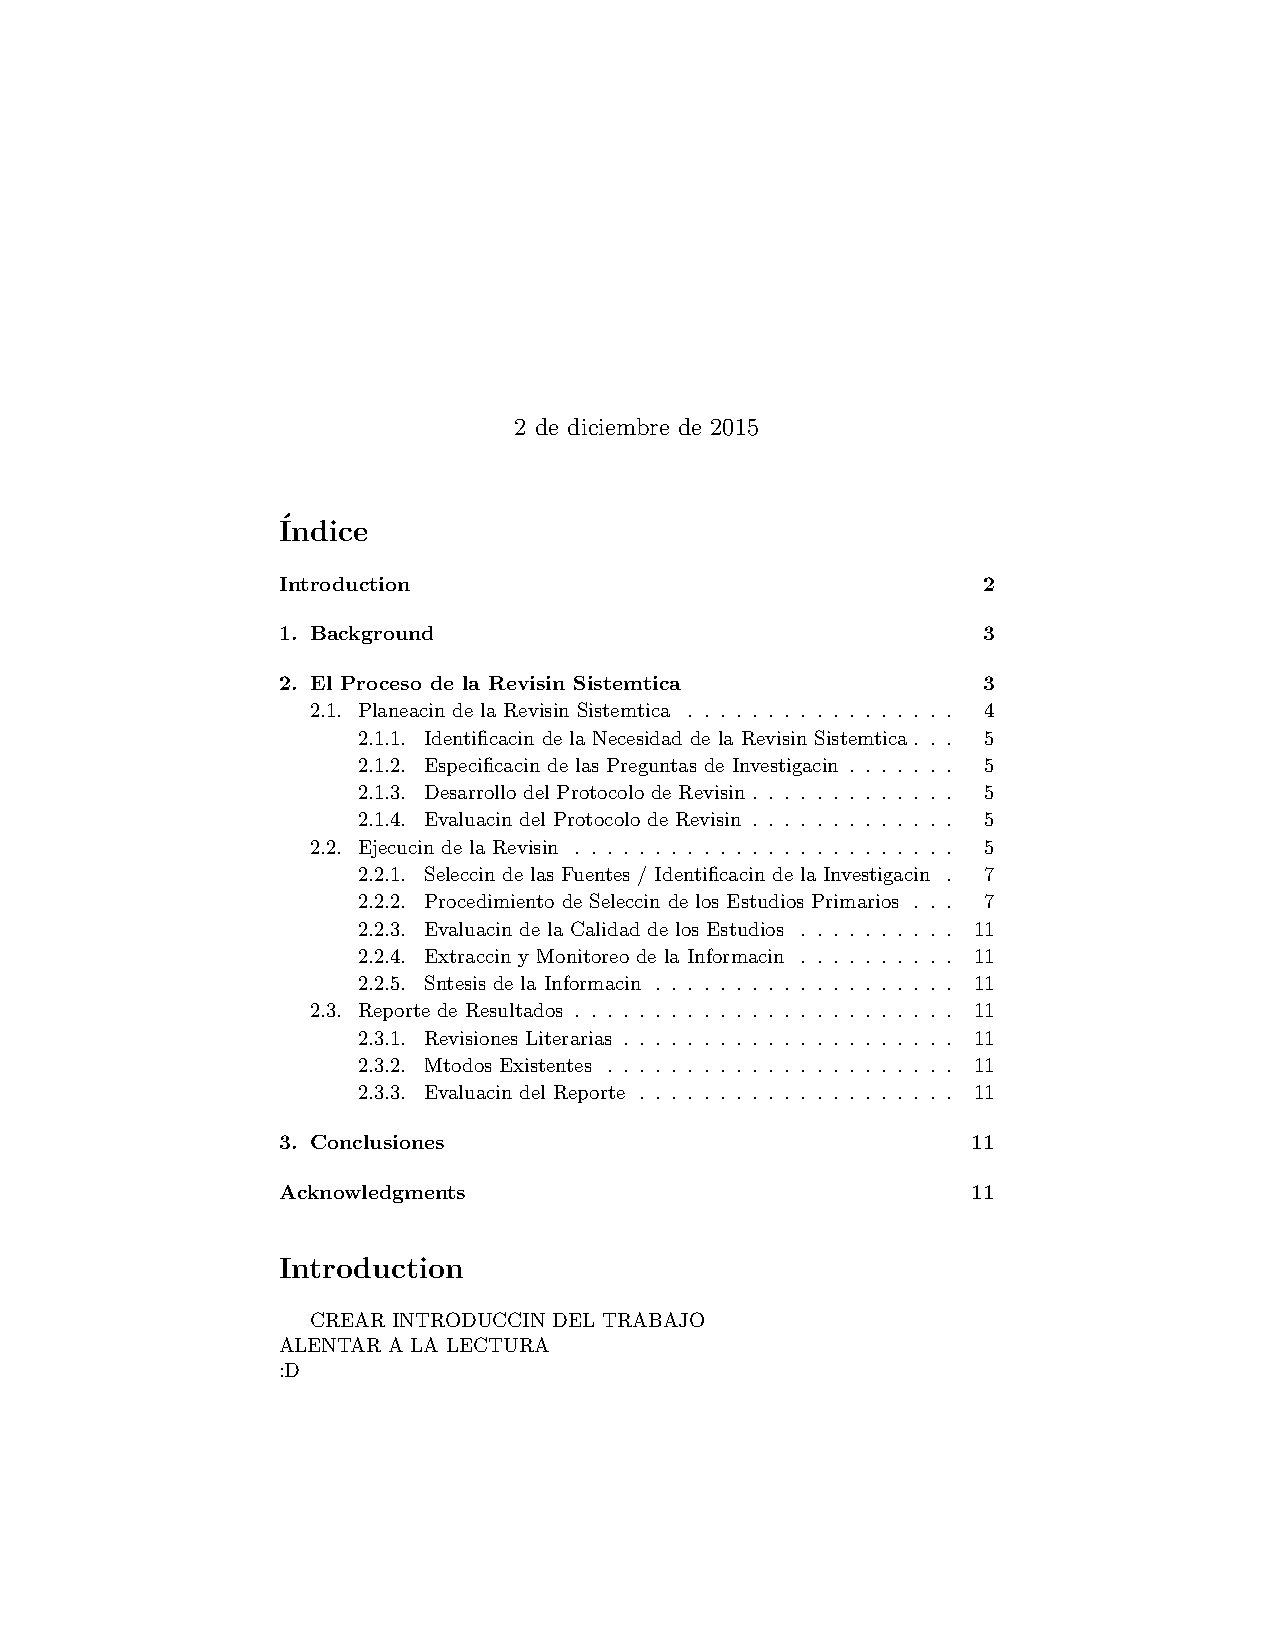
\includegraphics[width=0.8\linewidth]{test}
%\end{figure}
\end{frame}

%------------------------------------------------

\begin{frame}[fragile] % Need to use the fragile option when verbatim is used in the slide
\frametitle{Citation}
An example of the \verb|\cite| command to cite within the presentation:\\~

This statement requires citation \cite{p1}.
\end{frame}

%------------------------------------------------

\begin{frame}
\frametitle{References}
\footnotesize{
\begin{thebibliography}{99} % Beamer does not support BibTeX so references must be inserted manually as below
\bibitem[Smith, 2012]{p1} John Smith (2012)
\newblock Title of the publication
\newblock \emph{Journal Name} 12(3), 45 -- 678.
\end{thebibliography}
}
\end{frame}

%------------------------------------------------

\begin{frame}
\Huge{\centerline{The End}}
\end{frame}

%----------------------------------------------------------------------------------------

\end{document} 